\documentclass[a4paper,12pt]{article}
%\DeclareMathSizes{display size}{text size}{script size}{scriptscript size}.

\title{\vspace{-1.7 cm} Text Classification Notes}
\author{Gavin S. Hartnett}

\usepackage{url}
\usepackage{amssymb}
\usepackage{amsmath}
\usepackage[left=1.8cm,right=1.8cm,top=2cm,bottom=2.0cm,nohead]{geometry}
\usepackage[usenames]{color}
\usepackage{epsfig,latexsym,amsfonts,amsmath,amsthm,amssymb,amsbsy,multirow,slashed,color,mathrsfs,wasysym,textcomp,subfigure,wrapfig,comment}
\usepackage{framed} 
\usepackage{parskip}
\usepackage{graphicx,caption}

\renewcommand{\rmdefault}{phv} %Arial
\renewcommand{\sfdefault}{phv} %Arial 
\newcommand{\BibTeX}{{\sc Bib}\TeX}
\newcommand{\blue}[1]{\textcolor{blue}{#1}}
\newcommand{\red}[1]{\textcolor{red}{#1}}

\usepackage[skip=2pt,font=small]{caption}


\date{}
\begin{document}
\maketitle
\vspace{-0.5cm}
\abstract{Here are some notes on the various classification algorithms I used.}

%%%%%%%%%%%%%%%%%%%%%%%%%%%%%%%%%%%%%%%%%%%%%% Body %%%%%%%%%%%%%%%%%%%%%%%%%%%%%%%%%%%%%%%%%%%%%%
\section{Naive Bayes}
Let $c$ correspond to a class and $C$ be the set of all classes, and let $d$ schematically represent the features associated with a document. Given a document, we want to predict the class. To do so, we will estimate $P(c|d)$. If we know this for all $c \in C$, then we can simply take the most likely class as our prediction:
\begin{equation}
\hat{c}(d) = \text{argmax}_{c \in C} P(c|d) 
\end{equation}
Rather than modelling $P(c|d)$ directly, we will employ Bayes' theorem to write
\begin{equation}
P(c|d) = \frac{P(d|c) P(c)}{P(d)} \, .
\end{equation}
Here the hats indicate estimates. In the Naive Bayes approach we will model $P(d|c)$. $P(c)$ can be easily estimated from the data. $P(d)$ is difficult to model, but there is no need to have any knowledge of $P(d)$ for present purposes because it is independent of $c$. Therefore, 
\begin{equation}
\hat{c}(d) = \text{argmax}_{c \in C} P(d|c)P(c)
\end{equation}

In order to estimate the above probabilities we will make use of a training set of documents $D$. In this set the class assignments are known, $c(d)$. The first thing to estimate is
$P(c)$, the prior for each class. We'll simply take it to be the fraction of documents with class $c$:
\begin{equation}
\hat{P}(c) = \frac{1}{D} \sum_{d \in D} \delta_{c,c(d)} \, .
\end{equation}

The more difficult thing to estimate is $P(d|c)$. Now we need to be a bit more precise about what $d$ actually means. We want to represent a given document $d$ as a collection of $n$ features $x_i$, as in $d \rightarrow (x_1, x_2, ... , x_n)$. Exactly how this is achieved depends on the model and the assumptions being made.

First, in practice documents will undergo preprocessing to put them into a simple, common format, and to strip off unneccessary information. For example the cases might all be lowered, punctuation dropped, and stop words like 'and' removed. Second, we will make the so-called \textit{bag of words} assumption, which is to say the order of the words will be considered irrelevant. In this case, the $x_i$ will represent the words that show up in the training corpus $D$, and $(x_1, x_2, ... , x_n)$ will be a sparse integer-valued vector, wiht the integers denoting the number of times that word appeared in $D$. This means that now we want to estimate $P(c|x_1, x_2, ..., x_n)$. 

The Naive Bayes assumption is to assume that the features are all conditionally independent from one another. This means, for example, that
\begin{equation}
P(x_1 | x_2, ..., x_n; c) = P(x_1|c)\, . 
\end{equation}
Using this assumption, and the chain rule for conditional probabilities, $P(d|c)$ becomes
\begin{equation}
P(x_1, ..., x_n|c) = \prod_{i=1}^n P(x_i |c) \, .
\end{equation}
This is a very useful, but also strong assumption. The last part of the algorithm requires an estimate of $P(x_i|c)$. This is given by the average appearance of feature $x_i$ in class $c$. When the $x_i$ are word counts, this means that
\begin{equation}
\hat{P}(x_i | c) = \frac{\text{count}(x_i, c)}{\sum_i^n \text{count}(x_i, c)} \, ,
\end{equation}
where count$(x_i,c)$ is the number of times feature $x_i$ appears in class $c$. What if a word contains a feature (i.e. a word) not contained in the class $c$ training data? We'll take count$(y|c) =0$ for $y \neq x_i \forall i$.

This brings us to a big problem. If our classifier encounters a word $y$ it's never seen before in class $c$, then $P(d|c) \propto P(y|c) = 0$. This isn't good at all for 2 reasons. First, you might hope that in the event that a new word is encountered the classifier would assume uniform distribution for the prior. Secondly, if one conditional probability vanishes, the entire $P(c|d)$ vanishes also! So seeing one new word sends the whole probability to zero!

A remedy is to add a regulator that interpolates between the above expression and a uniform distribution, as in 
\begin{equation}
\hat{P}(x_i | c) = \frac{\alpha + \text{count}(x_i, c)}{n \alpha + \sum_i^n \text{count}(x_i, c)} \, ,
\end{equation}
In the event where the count vanishes, $\hat{P}(y|c) = 1/n$. This is known as Laplace smoothing. Often $\alpha = 1$ is taken, in which case this is sometimes known as $+1$ smoothing. 

\section{Maximum Entropy}
Let me derive some basic properties of the maximum entropy (MaxEnt) classifier.

Suppose we want to find the probability distribution $p(x)$ that 1) maximizes the entropy $H[p(x)] = - \int p(x) \ln p(x) dx$ and 2) obeys some constraints:
\begin{equation}
\int p(x) dx = 1, \qquad \int p(x) f_i(x) dx = F_i
\end{equation}
We can achieve this by introducing Lagrange multipliers, 
\begin{equation}
L[p(x); \lambda_0, \lambda_i] = H + \lambda_0 \left( \int p(x) dx - 1 \right) + \lambda_i \left( \int p(x) f_i dx = F_i \right) \, . 
\end{equation}
Solving for $\delta L/\delta p(x) = 0$ yields
\begin{equation}
p(x) = \exp\left(-(1+\lambda_0)-\lambda_i f_i(x) \right) \, .
\end{equation}
The Lagrange multipliers may then be solved for by solving $\partial L/\partial \lambda = 0$. The $\lambda_0$ straightforward to solve for,
\begin{equation}
e^{(1+\lambda_0)} = Z \equiv \int e^{-\lambda_i f_i(x)} dx \, \quad \Rightarrow \quad p(x) = Z^{-1} e^{-\lambda_i f_i(x)}
\end{equation}
Solving for the $\lambda_i$ is only possible when the $f_i(x)$ are known because the equation
\begin{equation}
F_i = \langle f_i(x) \rangle = Z^{-1} \int f_i(x) e^{-\lambda_i f_i(x)}
\end{equation}
must be inverted to get $\lambda_i(F)$. I will denote the solution(s) of this variational problem by $p^*(x; \lambda^*)$, although I will sometimes drop the $\lambda$ argument.

By solving these variational equations we get a stationary point of the entropy functional $p^*(x)$. It turns out that 1) there is only one stationary point and this is the global maximum, 2) if we solve the $\delta L/\delta p=0$ equation and consider the remaining variational problem in the $\lambda$'s, the problem is concave. I'm finding a hard time seeing a concrete derivation of this, so let me here collect some results from various sources and see if I can combine them to prove this.

\subsection{some properties}
\textbf{uniqueness} \\
Let's consider two distributions $p*(x)$ and some other distribution $p(x)$ that satisfies the constraints but may not fit the exponential form. We have
\begin{align}
H[p] &= - \int p(x) \ln p(x) dx = - \int p(x) \ln \left( \frac{p(x)}{p^*(x)} \right) dx - \int p(x) \ln p^*(x) dx \, \\
& = -D_{KL}(p || p^*) - \int p(x) \left[- \ln Z(\lambda^*) - \lambda_i^* f_i(x) \right] dx \\
& = -D_{KL}(p || p^*) - \int p^*(x) \left[  -\ln Z(\lambda^*) - \lambda_i^* f_i(x)  \right] dx \\
& = -D_{KL}(p || p^*) + H[p^*]
\end{align}
Here $D_{KL}$ is the Kullback-Liebler divergence. This divergence has the property $D_{KL}[p||p^*] \ge 0$ and is zero if and only if $p^* = p$. Because $H[p]\ge 0$, we can conclude that the global maximum of the entropy must occur for a distribution of the exponential form, $p*$. N.B. this doesn't seem too useful, because we previously derived under no assumptions at all that the stationary points take the exponential form.

A more useful result is as follows. If we suppose we have two distributions, $p^*$, $q^*$ which satisfied the constraints \textit{and} were of exponential form, then we can use this formula to conclude that $p^* = q^*$ because the derivation would then be symmetric between $p^*$ and $q^*$ and we would have
\begin{align}
& H[p^*] - H[q^*] = - D_{KL}[p^* || q^*] \le 0, \\
& H[q^*] - H[p^*] = - D_{KL}[q^* || p^*] \le 0, \\
\end{align}
and so $D_{KL}[p^* || q^*] = 0$, implying $p^* = q^*$. This result is much more useful--it says that there can only be 1 stationary point.
\\ \\
\textbf{convex/concave properties} \\
First, let's consider concavity. Convexity/concavity for a function $y(x)$ means that for $x_1 \le x_2$, and $t \in [0,1]$, 
\begin{align} 
& \text{convex:} \quad y(t x_1 + (1-t) x_2) \le t  y(x_1) + (1-t) y(x_2) \, , \\
& \text{concave:} \quad y(t x_1 + (1-t) x_2) \ge t  y(x_1) + (1-t) y(x_2) \, .
\end{align}
Clearly a linear function is both convex and concave. Also, a function is convex/concave if it's second derivative is everywhere positive/negative. I'm ignoring the distinction b/w strongly convex and generalizations to higher dimensions for now.
\\ \\
Next, I'll show that the log of the partition function $\ln Z(\lambda)$ (minus the free energy) is convex.
\begin{equation} 
\ln Z(t \lambda_1 + (1-t) \lambda_2) \le t \ln  Z(\lambda_1) + (1-t) \ln  Z(\lambda_2) \, .
\end{equation}
The derivation relies on H{\"o}lder's inequality, $ || f g ||_1 = ||f ||_p ||g ||_q$ for $1/p+1/q = 1$. 
\begin{align}
\ln Z(t \lambda_1 + (1-t) \lambda_2) &= \ln \int dx \left[ e^{-t \lambda_1 f} e^{-(1-t) \lambda_2 f} \right] \le \\
& \ln \left[ \int dx e^{-t p \lambda_1 f } \right]^{1/p} \left[ \int dx e^{-(1-t) q \lambda_2 f} \right]^{1/q} \, 
\end{align}
where the powers of $1/p, 1/q$ come from the definition of $||f||_p$. Set $p=1/t$ and $q=1/(1-t)$, and the convexivity inequality follows immediately. 
\\ \\
Next, consider the entropy. To show that it is concave, maybe the simplest thing is to take a second (variatonal) derivative:
\begin{equation}
\frac{\delta^2}{\delta p(x) \delta p(x')} H[p] = - \frac{1}{p(x')} \delta(x-x')
\end{equation}
which is negative in the sense that it's integral is negative. 

So if we consider the original, unconstrained Lagrangian, the $\lambda$-dependence is linear, so it is certainly concave in those directions, and the other term is the entropy, which is also concave in a functional sense. So this is very sloppy, but I've convinced myself.



\section{Evaluation}
The traditional way to evaluate performance is via classification error, the fraction of correctly classified tweets. For general classification problems, this is probably fine. In the case of sentiment analysis, it doesn't seem very in-line with what we want. Unlike classifying hand-written digits, where the classes have nothing to do with one another, here they are discrete coarse-grainings of a continuous sentiment variable. So the 3 different classes exist on a spectrum. 

A good error metric should make reference to what it is we're actually interested in measuring, which isn't whether a given tweet was classified correctly. Instead, we're interested in the sentiment density of a body of text, which we might define as
\begin{equation}
s = N^{-1} \sum_{i=1}^N S_i, \qquad S_i \in \{ -1, 0, 1 \} \, .
\end{equation}
Here $S_i$ is the sentiment for the $i$th tweet. The sentiment density $s$ gives us a measure of the sentiment contained in a body of tweets.

That the classification error isn't directly relevant to $s$ can be seen by imagining an extreme situation. Imagine our classifier always correctly identities positive and negative tweets, but always misidentifies neutral tweets. Let's say that half the time a neutral tweet is classified as positive, and the other half it's classified as negative. Depending on how many neutral tweets are in the tweet corpus, the classification error could be substantial, and yet we would have perfectly predicted the sentiment denisty (well, assuming the number of neutral tweets is even, otherwise we'd be off by a $O(N^{-1})$ amount). 

So it makes more sense to judge the efficacy of a model by the error in $s$. This will almost certainly depend on the distribution of sentiment in the corpus. To take another extreme case as an example, if our classifier always correctly identities neutral tweets, and always misidentifies positive and neutral tweets, we will still get a perfect measure of $s$ if the positive and negative tweets show up in equal number. Therefore, for cross-validation purposes, it would be convenient to have an ensemble of cross-validation data sets with differing rations of positive:neutral:negative tweets. Obtaining such an ensemble seems ridiculously time-consuming, and also inefficient, because we could start with a given CV set and produce smaller CV sets with different ratios by judiciously dropping tweets. In what follows, I'll work out how to do this.

\subsection{Ensemble Generation}
Let $N$ be the number of tweets in a given data set. Each tweet has a definite sentiment, so $N = N_+ + N_- + N_0$. It will be convenient to work with densities, so define $n_+ = N_+/N$, etc. The constraint is now tha the densities should add to 1:
\begin{equation}
1 = n_+ + n_- + n_0
\end{equation}
In addition to the above constraint, each density satisfies $0 \le n_i \le 1$. We can solve the constraint to eliminate $n_0$, in which case the domain is just the triangle $0\le n_+ \le 1$, $0 \le n_- \le 1$, $n_+ + n_- \le 1$. This is depicted in Fig.~\ref{fig:paramspace} below.

\begin{figure}[ht]
\centering
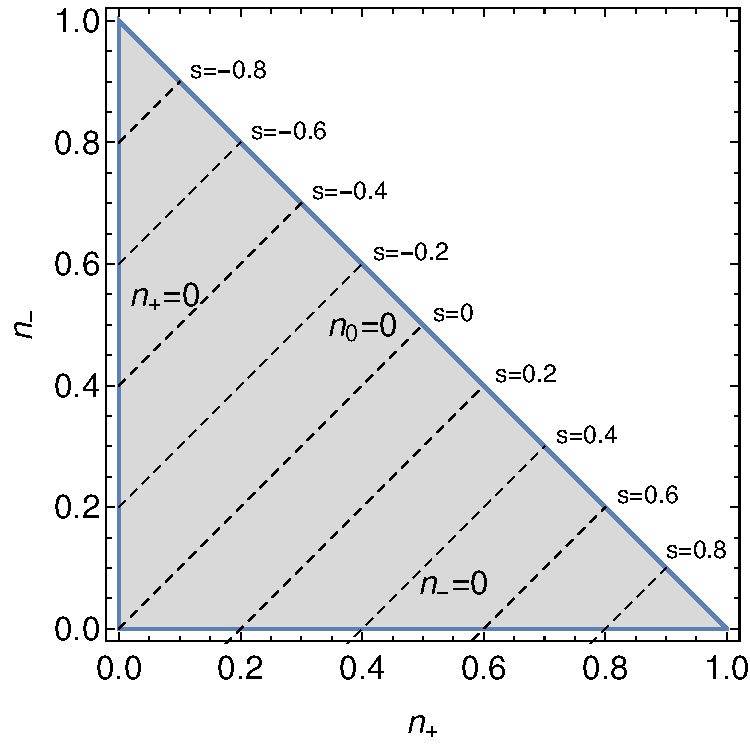
\includegraphics[width=.5\textwidth]{Figures/paramspace.pdf}
\captionsetup{width=0.8\textwidth}
\caption{The parameter space in the $(n_+, n_-)$ plane. The sides of the triangle correspond to one of the classes being absent, and the vertices correspond to two of the classes being absent (i.e. each tweet has the same sentiment). The dashed black lines are lines of constant sentiment, $s = n_+ - n_-$.}
\label{fig:paramspace}
\end{figure}  
While the parameter space is two-dimensional, the sentiment density only depends one paramter:
\begin{equation}
s = n_+ - n_- \, ,
\end{equation}
and so the parameter space can be ruled by lines of constant sentiment density. It's worth emphasizing that the error of a given model probably does depend on the full 2D parameter space.

Let's say that we start off with a given data set characterized by $N_+, N_-, N_0$. Let's drop a fraction $1-\alpha_i$ for the $i$-th class, i.e. $N_+' = \alpha_+ N_+$ and so on. The total size of the data set will also change, $N' = \alpha N$. The new densities will be given by
\begin{equation}
n_+' = \frac{\alpha_+}{\alpha} n_+, \qquad n_-' = \frac{\alpha_-}{\alpha} n_-, \qquad n_0' = \frac{\alpha_0}{\alpha} n_0 = 1 - n_+' - n_-'  \, .
\end{equation} 

In our case, we want to choose the $\alpha$'s so that the new densities will take some specified value. The simplest case is to cover the parameter space with a uniform $m \times m$ grid, which is to say:
\begin{equation}
n_+' = \frac{i}{m-1}, \qquad n_-' = \frac{j}{m-1} \, ,
\end{equation}
where $i,j = 0, ..., m-1$ subject to the constraint that $i+j \le m-1$. This is depicted below in Fig.~\ref{fig:paramspacegrid}.

\begin{figure}[ht]
\begin{center}
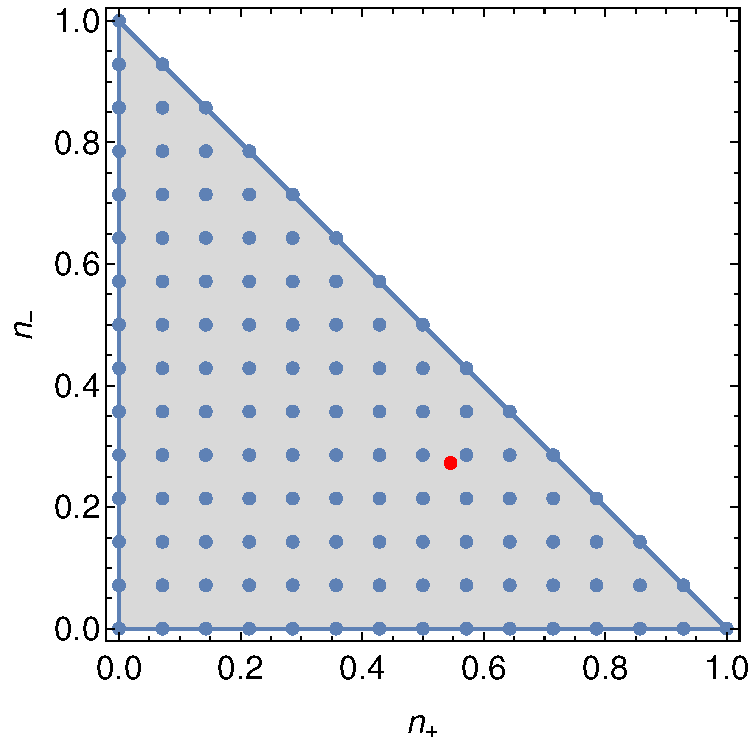
\includegraphics[width=.5\textwidth]{Figures/paramspacegrid.pdf}
\captionsetup{width=0.8\textwidth}
\caption{Starting from a given data set, represented by the red dot, an entire ensemble can be created by dropping tweets judiciously, with the new cv sets represented by the grid of blue dots.}
\label{fig:paramspacegrid}
\end{center}
\end{figure}  

This can be achieved by setting
\begin{equation}
\alpha_+ = \frac{\alpha}{n_+} \left(\frac{i}{m-1}\right), \qquad \alpha_- = \frac{\alpha}{n_-} \left(\frac{j}{m-1}\right) \qquad \alpha_0 = \alpha \left(\frac{1 - \frac{i+j}{m-1}}{1-n_+ - n_-} \right) \, .
\end{equation}
We have yet to specify $\alpha$, the total fraction of kept data. This is a free parameter that we will have to specify. Ideally, we would drop as little data as possible. If $\alpha$ is too large, then some of the fractions may exceed 1. By setting 
\begin{equation}
\alpha = \text{min} \left( n_+, n_-, n_0 \right)\, , 
\end{equation}
we can guarantee that the fractions are as large as possible without ever exceeding 1. 

With this grid, we can now compute the error in $s$ as a function of the statistics of the CV set, giving us a much more detailed understanding of the model's strenghts and weaknesses.



%%%%%%%%%%%%%%%%%%%%%%%%%%
%Bibliography
%%%%%%%%%%%%%%%%%%%%%%%%%%
\bibliography{refs}{}
\bibliographystyle{utphys}

\end{document}